\chapter{Implementation}

This chapter introduces some interesting implementation details and techniques, focusing mainly on the frontend but also mentioning the backend, including the spaced repetition algorithm.

\section{Frontend implementation}

This section presents the completed frontend application, illustrated with pictures, and then describes the solutions used during the implementation, highlighting the exciting features.

\subsection{The frontend application and screenshots}

\subsection{Project structure}

The project follows a flat folder structure hierarchy inspired by \texttt{The Go Standard Project Layout}\footnote{https://github.com/golang-standards/project-layout}. Figure \ref{fig:frontend-project-structure} shows this folder structure visually.

\begin{figure}[H]
    \centering
    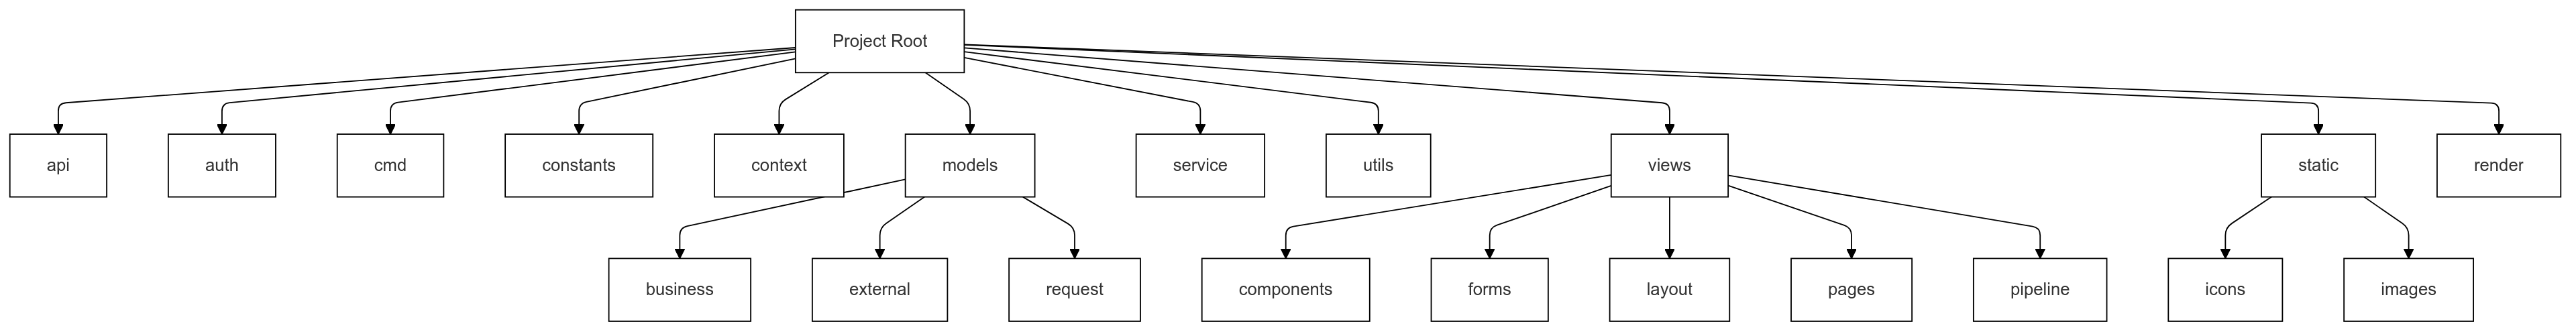
\includegraphics[width=0.8\textwidth, keepaspectratio]{figures/frontend-project-structure.png}
    \caption{Frontend project structure}
    \label{fig:frontend-project-structure}
\end{figure}

\textbf{api}: The \texttt{api} folder contains the endpoint handlers related to the pages and HTMX interactions.

\textbf{auth}: The \texttt{auth} folder contains the endpoint handlers related to the authentication function of the platform.

\textbf{cmd}: The folder \texttt{cmd} is a Go-specific folder containing the main functions. It is a common way to define the entry point of an application in \texttt{cmd/main.go}.

\textbf{constants}: The \texttt{constants} folder contains run-time constants; they wrap the provided environment variables and make them globally available for the application.

\textbf{context}: The \texttt{context} folder contains the custom context of the application. This context includes user information like a session ID and username.

\textbf{models}: The \texttt{models} folder contains Go representations of the data models in different layers and provides mappings between them. There are three layers of data: business, external, and request, which are separated into subfolders.

\textbf{service}: The \texttt{service} folder contains the ApiService, a proxy service providing access to the backend via function calls. This service is accessible through the custom context because the server calls usually require attaching the session ID to the request, and this service can do it automatically.

\textbf{utils}: The \texttt{utils} folder contains utils functions like generating gradient background from UUIDs and finding elements in lists.

\textbf{view}: The \texttt{view} folder contains the templ components and the generated Go code generated from them. They are also separated into subfolders based on their usage: \texttt{components}, \texttt{forms}, \texttt{layout}, \texttt{pages}, and \texttt{pipeline}.

\textbf{static}: The \texttt{static} folder is a regular webserver folder containing static resources for the application, such as scripts, images, and icons.

\textbf{render}: The \texttt{render} folder contains the configuration of the templ renderer and the render pipeline.

\subsection{Data models}

The application operates with three layers of data models. Each has a specific use case and can be mapped into other layer equivalents with mapping functions. These layers are the following: \texttt{business} used for doing the business logic, \texttt{external} used as Data Transfer Objects (DTO), and \texttt{request} used as communicating with the user. Listing \ref{lst:mapping-example} shows an example for mapping a quiz result object from \texttt{external} to \texttt{business} layer.

\begin{lstlisting}[caption=Mapping from external to business,label=lst:mapping-example]
func (result *QuizResult) MapToBusiness() (*business.QuizResult, error) {
    answerScores := make([]business.AnswerScore, 0, len(result.AnswerScores))
    for _, score := range result.AnswerScores {
        answerScore, err := score.MapToBusiness()
        if err != nil {
            return nil, err
        }
        answerScores = append(answerScores, *answerScore)
    }

    return &business.QuizResult{
        ID:           result.ID,
        SessionID:    result.SessionID,
        MaxScore:     result.MaxScore,
        Score:        result.Score,
        AnswerScores: answerScores,
    }, nil
}
\end{lstlisting}

The business layer objects are usually mappings from DTOs, with minor changes for effortless rendering. The DTOs are Go structs with \texttt{struct tags} used for parsing JSON objects. They are mostly the same as used on the backend. The request layer objects are similar to DTOs, but their \texttt{struct tags} help to map form data sent by the client instead of JSON sent by the server.

\subsection{Authentication}

\subsection{Rendering pipeline}

\subsection{Form handling}

\subsection{Backend integration}